\section{Постановка задачи}

\begin{frame}
    \frametitle{Постановка задачи}
    \begin{figure}
        \centering
        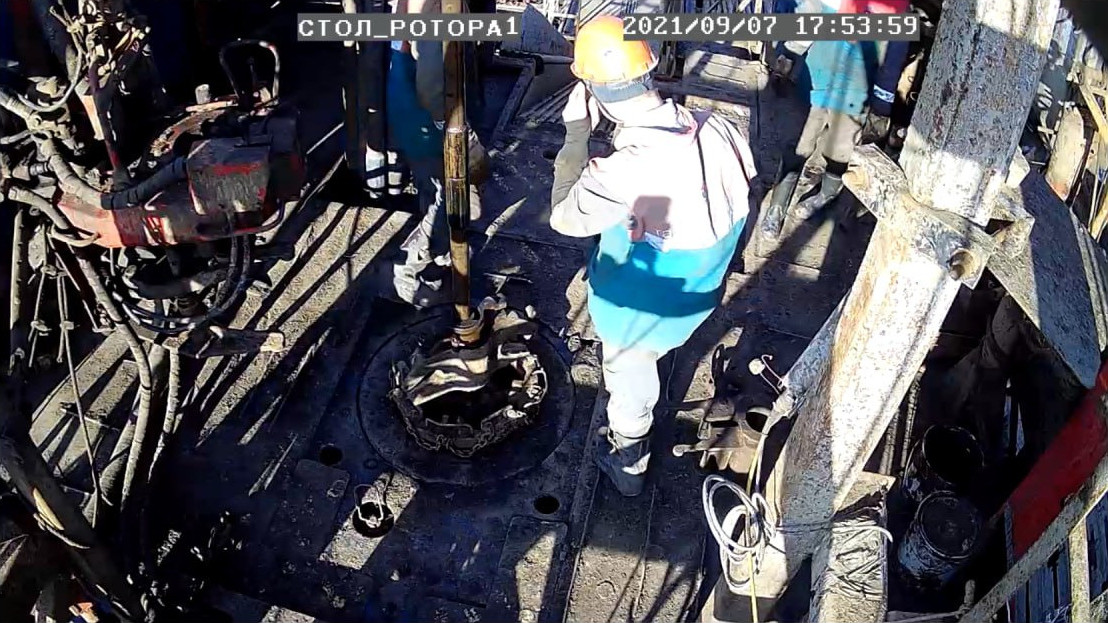
\includegraphics[width=1.0\textwidth,keepaspectratio]{problem_formulation_1}
    \end{figure}
\end{frame}

\begin{frame}
    \frametitle{Постановка задачи}
    Начальные предположения:
    \begin{itemize}
        \item Опасная зона для конкретной камеры задана заранее
        \item Детектируем только случай нахождения в опасной зоне без СИЗ
    \end{itemize}
\end{frame}

\begin{frame}
    \frametitle{Архитектура решения}
    \begin{figure}
        \centering
        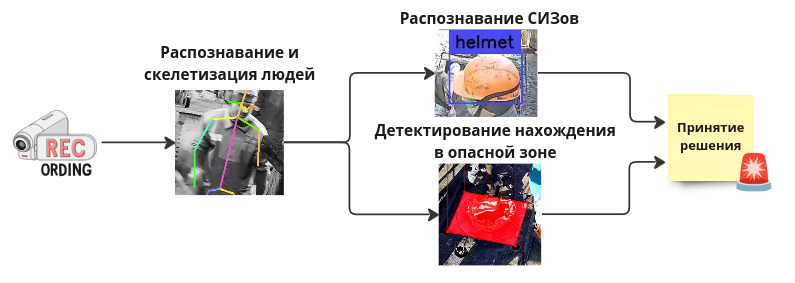
\includegraphics[width=1.1\textwidth,keepaspectratio]{general_architecture}
    \end{figure}
\end{frame}
